\documentclass{article} % For LaTeX2e
\usepackage{nips13submit_e,times}
\usepackage{hyperref}
\usepackage{url}
%\documentstyle[nips13submit_09,times,art10]{article} % For LaTeX 2.09


\usepackage{amsmath, amssymb, color}
%\usepackage{amsthm}
\usepackage{hyperref, url}
\usepackage{graphicx}               % Use pdf, png, jpg, or eps§ with pdflatex; use eps in DVI mode. TeX will automatically convert eps --> pdf in pdflatex



% New environment part
\newtheorem{definition}{Definition}
\newtheorem{assumption}{Assumption}
\newtheorem{fact}{Fact}
\newtheorem{theorem}{Theorem}%[section]
\newtheorem{lemma}[theorem]{Lemma}
\newtheorem{corollary}[theorem]{Corollary}
\newtheorem{proposition}[theorem]{Proposition}
\newtheorem{claim}[theorem]{Claim}
\newtheorem{remark}{Remark}
\newtheorem{example}{Example}
% Need the environment Proof ? Please use the following:
% {\noindent\bf Proof.}  ...........................  $\hfill \square$\\

% Bold type part.
\newcommand{\ba}{\mbox{\boldmath $a$}}
\newcommand{\bb}{\mbox{\boldmath $b$}}
\newcommand{\bc}{\mbox{\boldmath $c$}}
\newcommand{\bd}{\mbox{\boldmath $d$}}
\newcommand{\be}{\mbox{\boldmath $e$}}
\newcommand{\bff}{\mbox{\boldmath $f$}} %NOTICE!
\newcommand{\bg}{\mbox{\boldmath $g$}}
\newcommand{\bh}{\mbox{\boldmath $h$}}
\newcommand{\bo}{\mbox{\boldmath $o$}}
\newcommand{\bp}{\mbox{\boldmath $p$}}
\newcommand{\bq}{\mbox{\boldmath $q$}}
\newcommand{\br}{\mbox{\boldmath $r$}}
\newcommand{\bs}{\mbox{\boldmath $s$}}
\newcommand{\bt}{\mbox{\boldmath $t$}}
\newcommand{\bu}{\mbox{\boldmath $u$}}
\newcommand{\bv}{\mbox{\boldmath $v$}}
\newcommand{\bw}{\mbox{\boldmath $w$}}
\newcommand{\bx}{\mbox{\boldmath $x$}}
\newcommand{\by}{\mbox{\boldmath $y$}}
\newcommand{\bz}{\mbox{\boldmath $z$}}
\newcommand{\bzero}{\mbox
%{\Large 
{\boldmath $0$}}
%}

\newcommand{\bA}{\mbox{\boldmath $A$}}
\newcommand{\bB}{\mbox{\boldmath $B$}}
\newcommand{\bC}{\mbox{\boldmath $C$}}
\newcommand{\bD}{\mbox{\boldmath $D$}}
\newcommand{\bI}{\mbox{\boldmath $I$}}
\newcommand{\bM}{\mbox{\boldmath $M$}}
\newcommand{\bU}{\mbox{\boldmath $U$}}
\newcommand{\bV}{\mbox{\boldmath $V$}}
\newcommand{\bW}{\mbox{\boldmath $W$}}
\newcommand{\bX}{\mbox{\boldmath $X$}}
\newcommand{\bY}{\mbox{\boldmath $Y$}}
\newcommand{\bZ}{\mbox{\boldmath $Z$}}

\newcommand{\balpha}{\mbox{\boldmath $\alpha$}}
\newcommand{\bbeta}{\mbox{\boldmath $\beta$}}
\newcommand{\btheta}{\mbox{\boldmath $\theta$}}
\newcommand{\bgamma}{\mbox{\boldmath $\gamma$}}
\newcommand{\bdelta}{\mbox{\boldmath $\delta$}}
\newcommand{\bmu}{\mbox{\boldmath $\mu$}}
\newcommand{\bepsilon}{\mbox{\boldmath $\epsilon$}}
\newcommand{\blambda}{\mbox{\boldmath $\lambda$}}
\newcommand{\btau}{\mbox{\boldmath $\tau$}}
\newcommand{\bsigma}{\mbox{\boldmath $\sigma$}}
\newcommand{\bSigma}{\mbox{\boldmath $\Sigma$}}

% Specific math notation:
\newcommand{\real}[1]{\mbox{$\mathbb{R}^{#1}$}}
\newcommand{\prob}{\mbox{$\mathbb{P}$}}
\newcommand{\expect}{\mbox{$\mathbb{E}$}}
\newcommand{\var}{\mbox{$\mathbb{V}$}}
\newcommand{\compl}[1]{\mbox{$\mathbb{C}^{#1}$}}
\newcommand{\realN}[1]{\mbox{$\real{I_1 \times I_2 \times \dots \times I_{#1}}$}}
\newcommand{\complN}[1]{\mbox{$\compl{I_1 \times I_2 \times \dots \times I_{#1}}$}}
%\newcommand{\natural}{\mbox{$\mathbb{N}$}}

% Enumerate part
\newcommand{\V}[1]{\mbox{\boldmath $#1$}}
\newcommand{\RV}[1]{\mbox{\boldmath $\tilde{#1}$}}
\newcommand{\rv}[1]{\tilde{#1}}
\newcommand{\OPT}{{\mbox{OPT}}}
\newcommand{\SP}{{\tt{SP}}}
\newcommand{\CVX}{{\tt{CVX}}}
\newcommand{\LP}{{\tt{LP}}}
\newcommand{\D}{{\tt{D}}}
\newcommand{\ALG}{\tt{ALG}}
\newcommand{\cT}{{\cal T}}

%Added on Feb 23, 2015: Roman numbers, chapters, DEFINE format
\newcommand{\rmnum}[1]{\romannumeral #1} % Roman small letter
\newcommand{\Rmnum}[1]{\uppercase\expandafter{\romannumeral #1}} % Roman capital letter
\usepackage[raggedright]{titlesec}% 可换为 raggedleft  raggedright
\titleformat{\chapter}{\centering\Huge\bfseries}{Chapter \Rmnum{\thechapter} }{1em}{} % in book format
\newcommand{\df}{\bfseries \em}  % DEFINE format for text

%Added on April 30th, 2015: 
\usepackage{mathrsfs} %math-script format, then use \mathscr{F} 
\usepackage{enumerate} % change the symbols in enumerate
\graphicspath{{figures/}}  %图片路径

%Added on Jul 11th, 2015:
\newcommand{\tensorA}{\mbox{\boldmath $\mathcal{A}$}}
\newcommand{\tensorD}{\mbox{\boldmath $\mathcal{D}$}}
\newcommand{\tensorE}{\mbox{\boldmath $\mathcal{E}$}}
\newcommand{\tensorF}{\mbox{\boldmath $\mathcal{F}$}}
\newcommand{\tensorG}{\mbox{\boldmath $\mathcal{G}$}}
\newcommand{\tensorI}{\mbox{\boldmath $\mathcal{I}$}}
\newcommand{\tensorU}{\mbox{\boldmath $\mathcal{U}$}}
\newcommand{\tensorV}{\mbox{\boldmath $\mathcal{V}$}}
\newcommand{\tensorX}{\mbox{\boldmath $\mathcal{X}$}}
\newcommand{\tensorY}{\mbox{\boldmath $\mathcal{Y}$}}
\usepackage{multirow}
\usepackage{amsmath} 
\usepackage{stmaryrd}
\usepackage{float}
\usepackage{graphicx}
\usepackage{subfigure}
\usepackage{xcolor} 
\DeclareMathOperator*{\argmin}{argmin}

\usepackage{color}
\newcommand{\tbw}{\bigskip \mbox{\color{red} {\df (TBW) }}\bigskip}

\newcommand{\hide}[1]{}
\newcommand{\hao}[1]{{\color{red} [[Hao: #1]]}}



\newcommand{\hasPageBreak}{\newpage}
%\newcommand{\hasPageBreak}{}


% Added on Dec 8th, 2015: listings
\usepackage{listings}

% Added on March 9th, 2016: algorithm
\usepackage{algorithm} 
\usepackage{algorithmic}
\renewcommand{\algorithmicrequire}{\textbf{Input:}}
\renewcommand{\algorithmicensure}{\textbf{Output:}}





\title{Aiding Sentiment Evaluation with Social Network}


\author{
Pengfei Gao, Fan Yang, Hao Yin
\thanks{Each member contributes equally, and names are put in alphabetic order.} \\
Institute for Computational and Mathematical Engineering\\
Stanford University\\
Stanford, CA 94305 \\
\texttt{\{pfgao, fanfyang, yinh\}@stanford.edu}
}

% The \author macro works with any number of authors. There are two commands
% used to separate the names and addresses of multiple authors: \And and \AND.
%
% Using \And between authors leaves it to \LaTeX{} to determine where to break
% the lines. Using \AND forces a linebreak at that point. So, if \LaTeX{}
% puts 3 of 4 authors names on the first line, and the last on the second
% line, try using \AND instead of \And before the third author name.

\newcommand{\fix}{\marginpar{FIX}}
\newcommand{\new}{\marginpar{NEW}}

\nipsfinalcopy % Uncomment for camera-ready version

\begin{document}


\maketitle

\begin{abstract}
Some abstract
\end{abstract}

\section{Introduction}
Milestone report is seen in Section 2. For reader's reference, we give an introduction of our project in this section.


In this project, we are going to explore different methods that utilize social network information in sentiment analysis with deep learning. Network structure is useful and informative in NLP-related task as people within each community may have their own ``jargon'' in expressing ideas and sentiments. 


\subsection*{Data description}
We obtained the data used by \cite{yang2017attention}. The data consists of a collection of tweets as well as some network information on Twitter. For each tweet sample, we have one tweet ID, one user ID, a sentiment label (positive, neutral, negative), and the tweet content itself. For example, the following are two examples of our data samples.
\begin{verbatim}
261140278944088066	17572408	negative	@USER may i have an industrial revolution ...
237571817550786563	727519172	neutral	@USER i told you shane would get his 5th-star ...
\end{verbatim}
We have three networks, i.e., FOLLOWER, MENTION and RETWEET network which have been explained in details by
\cite{yang2017attention}.





\subsection*{Methodology}
%Methodology/Algorithm: What method or algorithm are you proposing? If there are existing implementations, will you use them and how? How do you plan to improve or modify such implementations?

Our project will start from the method proposed by \cite{yang2017attention}, which is summarized in Figure \ref{Fig:Flow} (black lines). The model consider the author information and sentence information separately: each node (author) in the network is assigned an embedding vector using the LINE algorithm (\cite{tang2015line}), and then is (softly) assigned each cluster on the network based on the embedding. Each cluster has its own model, which is a CNN model combined with max pool layer. This model provides a baseline in our project.

\begin{figure}[htbp] %  figure placement: here, top, bottom, or page
   \centering
   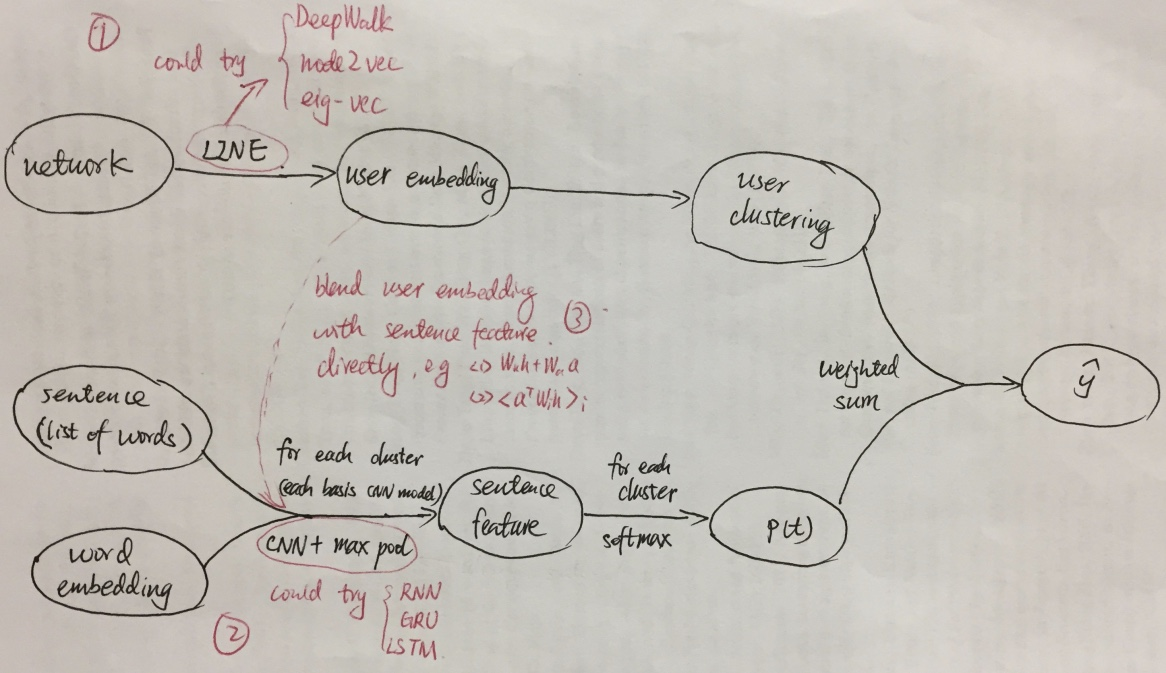
\includegraphics[width=5.2in]{flow.jpg} 
   \caption{General Methodology}
   \label{Fig:Flow}
\end{figure}



We are going to extend this model in three aspects, as is illustrated in the red lines in Figure \ref{Fig:Flow}. To be specific, 
\begin{enumerate}   [(1)]
%\setcounter{enumi}{3}
\item Using other node embedding methods in network analysis, such as \textit{DeepWalk} (\cite{perozzi2014deepwalk}) and \textit{node2vec} (\cite{grover2016node2vec});
\item Explore other methods to combine author information and sentence information, especially the bilinear form $a^T W h$ which measures the interaction between author and sentence. Here $a$ is the author embedding and $h$ is the sentence embedding.
\item Explore other models in sentiment analysis, such as RNN, GRU, and LSTM.
\end{enumerate}

\section{Progress}
As is advised by our project mentor Will Hamilton, since CNN is the current state-of-the-art model for sentiment analysis, we are going to focus on (1) and (2) above, and only work on part (3) if time permits. 

For part (1), we have already computed the embedding using \textit{DeepWalk}. Using the original model and implementation, this embedding does not outperform the existing result which uses the LINE embedding. We have just finished the embedding using \textit{node2vec}, and have not examined it with the existing result.
We intended to computed the embedding using Azure, but we experienced some issue in uploading our network edgelist files. We end up using CORN, which takes roughly 50 hours to finish.


For part (2), the original implementation uses Keras. We have just read through and understand all of their code, which can be finished in 10 minutes using personal computer CPU. 
We are contacting the authors for exact seeds to reproduce the results in the paper, and after that we are going to incorporate the author-sentence interaction feature into the existing model. 

%All our code (the baseline model) in hand can be implemented and finished in ten minutes using personal computer CPU, so we haven't implemented them on


\section{Results}

\begin{table}[htbp]
\begin{center}
\begin{tabular}{|c|c|c c c c|}
\hline
Embedding method & CNN & DeepWalk & LINE & node2vec & random\\
\hline
Dev2013  & 68.85 & 67.71 & \textbf{69.51} & 68.58 & 68.50 \\
\hline
Test2013  & 69.53 & 67.58 & \textbf{69.67} & 68.58 & 68.49 \\
Test2014  & \textbf{72.41} & 71.46 & 71.44 & 71.46 & 71.69 \\
Test2015  & 64.40 & \textbf{64.71} & 64.57 & 64.25 & 63.50 \\
\hline
Avg test sets & \textbf{68.78}& 67.92 & 68.56  & 68.10 & 67.89 \\
\hline
\end{tabular}
\end{center}
\caption{Prediction performance on each Dev and Test Sets. }
\label{Tb:}
\end{table}%



\bibliographystyle{ormsv080} 
\bibliography{Bibli}

\end{document}
